% 1962 年全国卷第 5 题：圆内接平行四边形为矩形。
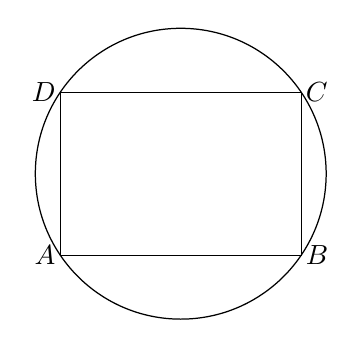
\begin{tikzpicture}[scale=0.9, line width=0.45pt,
  every node/.style={inner sep=1.5pt}]
  \coordinate (A) at (-1.7,-1.15);
  \coordinate (B) at (1.7,-1.15);
  \coordinate (C) at (1.7,1.15);
  \coordinate (D) at (-1.7,1.15);
  \draw (0,0) circle (2.052);
  \draw (A)--(B)--(C)--(D)--cycle;
  \node[anchor=east] at (A) {$A$};
  \node[anchor=west] at (B) {$B$};
  \node[anchor=west] at (C) {$C$};
  \node[anchor=east] at (D) {$D$};
\end{tikzpicture}
